%\SweaveUTF8




\setkeys{Gin}{width=\textwidth}

\begin{Problem}[One-stage cluster sampling]
    The California Academic Performance Index (API) was a measure of school
    performance based on standardized tests. API scores ranged from 200 to
    1,000, with higher values indicating better performance. The last API
    report was produced in 2013.

    \vspace{0.25em}

    The API data are included in the \code{survey} package and can be loaded
    with \code{data(api)}. We use the one-stage cluster sample
    \code{apiclus1}. A simple random sample of $n = 15$ school districts was
    drawn from $N = 757$ districts, and all schools in the selected districts
    were observed.

    \vspace{0.25em}

    The survey design is specified as follows:

\begin{Scode}
dn_api <- svydesign(id = ~dnum, weights = ~pw, fpc = ~fpc, data = apiclus1)
\end{Scode}

    Here, \code{dnum} identifies the school district, \code{pw} contains the
    design weights, and \code{fpc} contains the finite-population correction
    for sampling districts. We focus on \code{api00}, the API score in 2000.

\begin{Subtask}
    %---------------------------------------------------------------------------
    \item Estimate the population mean API score in 2000. Also compute the
        design effect by calling \code{svymean()} with \code{deff = TRUE}.

    \begin{Solution}
        Load the data and define the survey design:

\begin{Schunk}
\begin{Sinput}
> library("survey")
> data(api)
> dn_api <- svydesign(id = ~dnum, weights = ~pw, fpc = ~fpc, data = apiclus1)
\end{Sinput}
\end{Schunk}

        The estimated mean and its design effect are:

\begin{Schunk}
\begin{Sinput}
> mean_api <- svymean(~api00, dn_api, deff = TRUE)
> mean_api
\end{Sinput}
\begin{Soutput}
         mean      SE   DEff
api00 644.169  23.542 9.3459
\end{Soutput}
\end{Schunk}


        The design effect is about 9.3. Thus, the
        183 sampled schools contain roughly as much information about
        the population mean as an SRS of
        20 schools. The loss of efficiency is caused mainly
        by the similarity of schools within the same district.
    \end{Solution}

    %---------------------------------------------------------------------------
    \item Estimate the 25th percentile, median, and 75th percentile of the API
        score in 2000. Use

\begin{Scode}
svyquantile(x, design, quantiles, ...)
\end{Scode}

    \begin{Solution}
        We estimate all three quartiles at once:

\begin{Schunk}
\begin{Sinput}
> q_api <- svyquantile(~api00, dn_api, quantiles = c(0.25, 0.5, 0.75))
> q_api
\end{Sinput}
\begin{Soutput}
$api00
     quantile ci.2.5 ci.97.5       se
0.25      552    492     627 31.47166
0.5       652    561     714 35.66788
0.75      719    696     777 18.88300

attr(,"hasci")
[1] TRUE
attr(,"class")
[1] "newsvyquantile"
\end{Soutput}
\end{Schunk}


        The estimated median is 652. Its 95\,\% confidence interval
        is 561 to 714.
    \end{Solution}

    %---------------------------------------------------------------------------
    \item The California State Board of Education used an API score of 800 as
        a performance target. Estimate the proportion of schools with an API
        score below 800. Use

\begin{Scode}
svycdf(formula, design, ...)
\end{Scode}

    \begin{Solution}
        \code{svycdf()} estimates the population cumulative distribution
        function:

\begin{Schunk}
\begin{Sinput}
> F_hat <- svycdf(~api00, dn_api)
\end{Sinput}
\end{Schunk}

        Since API scores are integer-valued, the proportion below 800 is
        $\widehat F(799)$:

\begin{Schunk}
\begin{Sinput}
> p_below <- F_hat[[1]](799)
> p_below
\end{Sinput}
\begin{Soutput}
[1] 0.9234973
\end{Soutput}
\end{Schunk}

        Thus, about 92\,\% of schools have an API
        score below the target.

\begin{Schunk}
\begin{Sinput}
> plot(F_hat[[1]])
> abline(v = 800, lwd = 2)
\end{Sinput}
\end{Schunk}

        \begin{figure}[tbp]
            \centering
            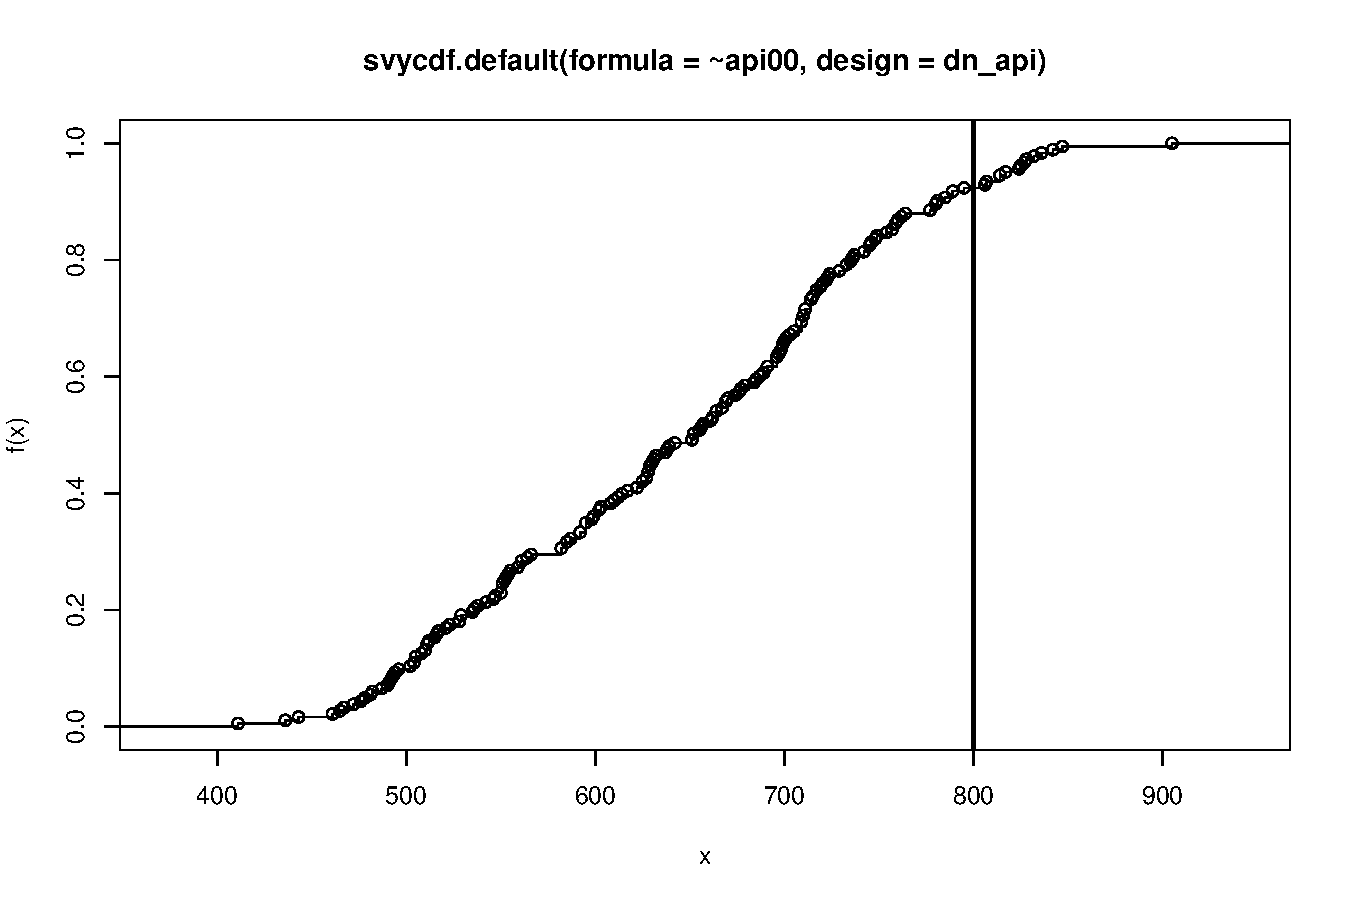
\includegraphics{problems/fig-cdf}
        \end{figure}
    \end{Solution}
\end{Subtask}
\end{Problem}
